\documentclass[a4, 10pt]{article}

\usepackage{balance}
\usepackage{amsmath,amssymb,psfrag,color,pbox,subfigure,graphicx,times}
%\usepackage[font={sf,bf}, size=small]{caption}
\setlength{\parindent}{0pt}
\setlength{\parskip}{1ex plus 0.5ex minus 0.2ex}
\renewcommand{\theenumi}{Ex. \arabic{enumi}}

\title{Exercise 2: Simultaneous Localization and Mapping using the
  Extended Kalman Filter}

\begin{document}
\maketitle

\section{Introduction}
One important aspect of robotic navigation is the ability to fuse
multiple sources of data. In the case of a mobile robot, we might have
a number of sensors telling us our current position. Each of these
sensors is subject to noise and errors of various kinds. Some sources
of position data, such as triangulated range and bearing observations
to known targets, are often quite noisy and subject to short term
errors. Other position information, such as odometry, is subject
to an accumulation of errors that result from inaccuracies in our
model and noise on the control lines. The fusion of these two sources
of data can, however, give us much better results since one is good
over the long term while the other is fairly reliable for predicting
our position over a short distance.

In this exercise, you will implement the Extended Kalman Filter (EKF)
for Simultaneous Localization and Mapping in Matlab.  Large parts of the code
are provided, but you need to implement parts of the transition model
(also termed prediction step) and the sensor model.


%
%\begin{equation}
%\mathbf{U}_{0:k} = \left\{\mathbf{u}_0,\dots, \mathbf{u}_{k}\right\} = \left\{ \mathbf{U}_{0:k-1},\mathbf{u_k}\right\}
%\mathbf{Z}_{0:k} = \left\{\mathbf{z}_0,\dots, \mathbf{z}_{k}\right\} = \left\{ \mathbf{Z}_{0:k-1},\mathbf{z_k}\right\}
%
%\end{equation}
%\section{Exercises}
%\begin{equation}
%\mathbf{x}_{k} = \left[  \begin{array}{c}
%\mathbf{x}_{v_{k}} \\
%m_{1} \\
%\dots\\
%m_{n}\\
%\end{array}
%\right]
%\end{equation}
%

The position of the robot and the landmarks in the map are contained
in the state vector:
\begin{equation}
\mathbf{x}_{k} = \left[  \begin{array}{c}
\mathbf{x}_{v_k}\\
m_{1} \\
\dots\\
m_{n}\\
\end{array}
\right]
\end{equation}
where $\mathbf{x}_{v_k}$ is the current vehicle state we are
estimating in the prediction stage. $m_i$ is the position of landmark
$i$ in the map. For clarity $\mathbf{x}_{v_{k}}$  can be decomposed as: 
\begin{equation}
\mathbf{x}_{v_{k}} = \{x_{v_{k}},y_{v_{k}} ,\psi_{v_{k}} \}^T
\end{equation}
where $x_{v_{k}}$ and $y_{v_{k}}$ are the x- and y-position of the
robot and $\psi_{v_{k}}$ is the orientation of the robot.

\subsection{Prediction Stage}
In the prediction stage we will use a simple bicycle vehicle model which appears in Figure~\ref{f:motion}. Vehicle control signals consist of a velocity and  a steering angle that can be retrieved from the robot. The vehicle model and update equations are included here for your implementation in the code.

The state vector in this step looks like:
\begin{equation}
\mathbf{x}_{k} = \left[  \begin{array}{c}
\mathbf{x}_{v_k}\\
m_{1} \\
\dots\\
m_{n}\\
\end{array}
\right]
\end{equation}

In the prediction step we want to update the position of the robot in
the state vector and the uncertainties in the covariance matrix. The
position of the robot is updated using the wheel direction and the
velocity of the robot:

\begin{equation}
\mathbf{x}_{v_k} = 
\begin{array}{c}
x_{v_{k}}\\
y_{v_{k}}\\
\psi_{v_{k}}
\end{array}
\mathbf{f}_v(\mathbf{x}_{v_{k-1}}, \mathbf{u}_k) = \left[
\begin{array}{c}
x_{v_{k-1}} + V_k \Delta T \cos(\psi_{v_{k-1}} + \gamma_k) \\
y_{v_{k-1}} + V_k \Delta T \sin(\psi_{v_{k-1}} + \gamma_k) \\
\psi_{v_{k-1}} + {V_k \Delta T \over B} \sin(\gamma_k)
\end{array}
\right]
\end{equation}
where $x_{v_{k-1}}$, $y_{v_{k-1}}$ are the xy position of the robot at time
$k-1$ and
where $V_k$ is the velocity control input and $\gamma_k$ is the
steering angle input and $B$ is the wheel base of the vehicle and
$\psi_{v_{k-1}} $ is orientation from the current head of the SLAM
state vector. 

In the matlab code you will work with, the state vector is contained
in the vector \verb|XX|. The robot's xy and angle position are in
\verb|XX(1:3)|. The other elements in the array contain the landmark
positions.

\begin{figure}[h]
\begin{center}
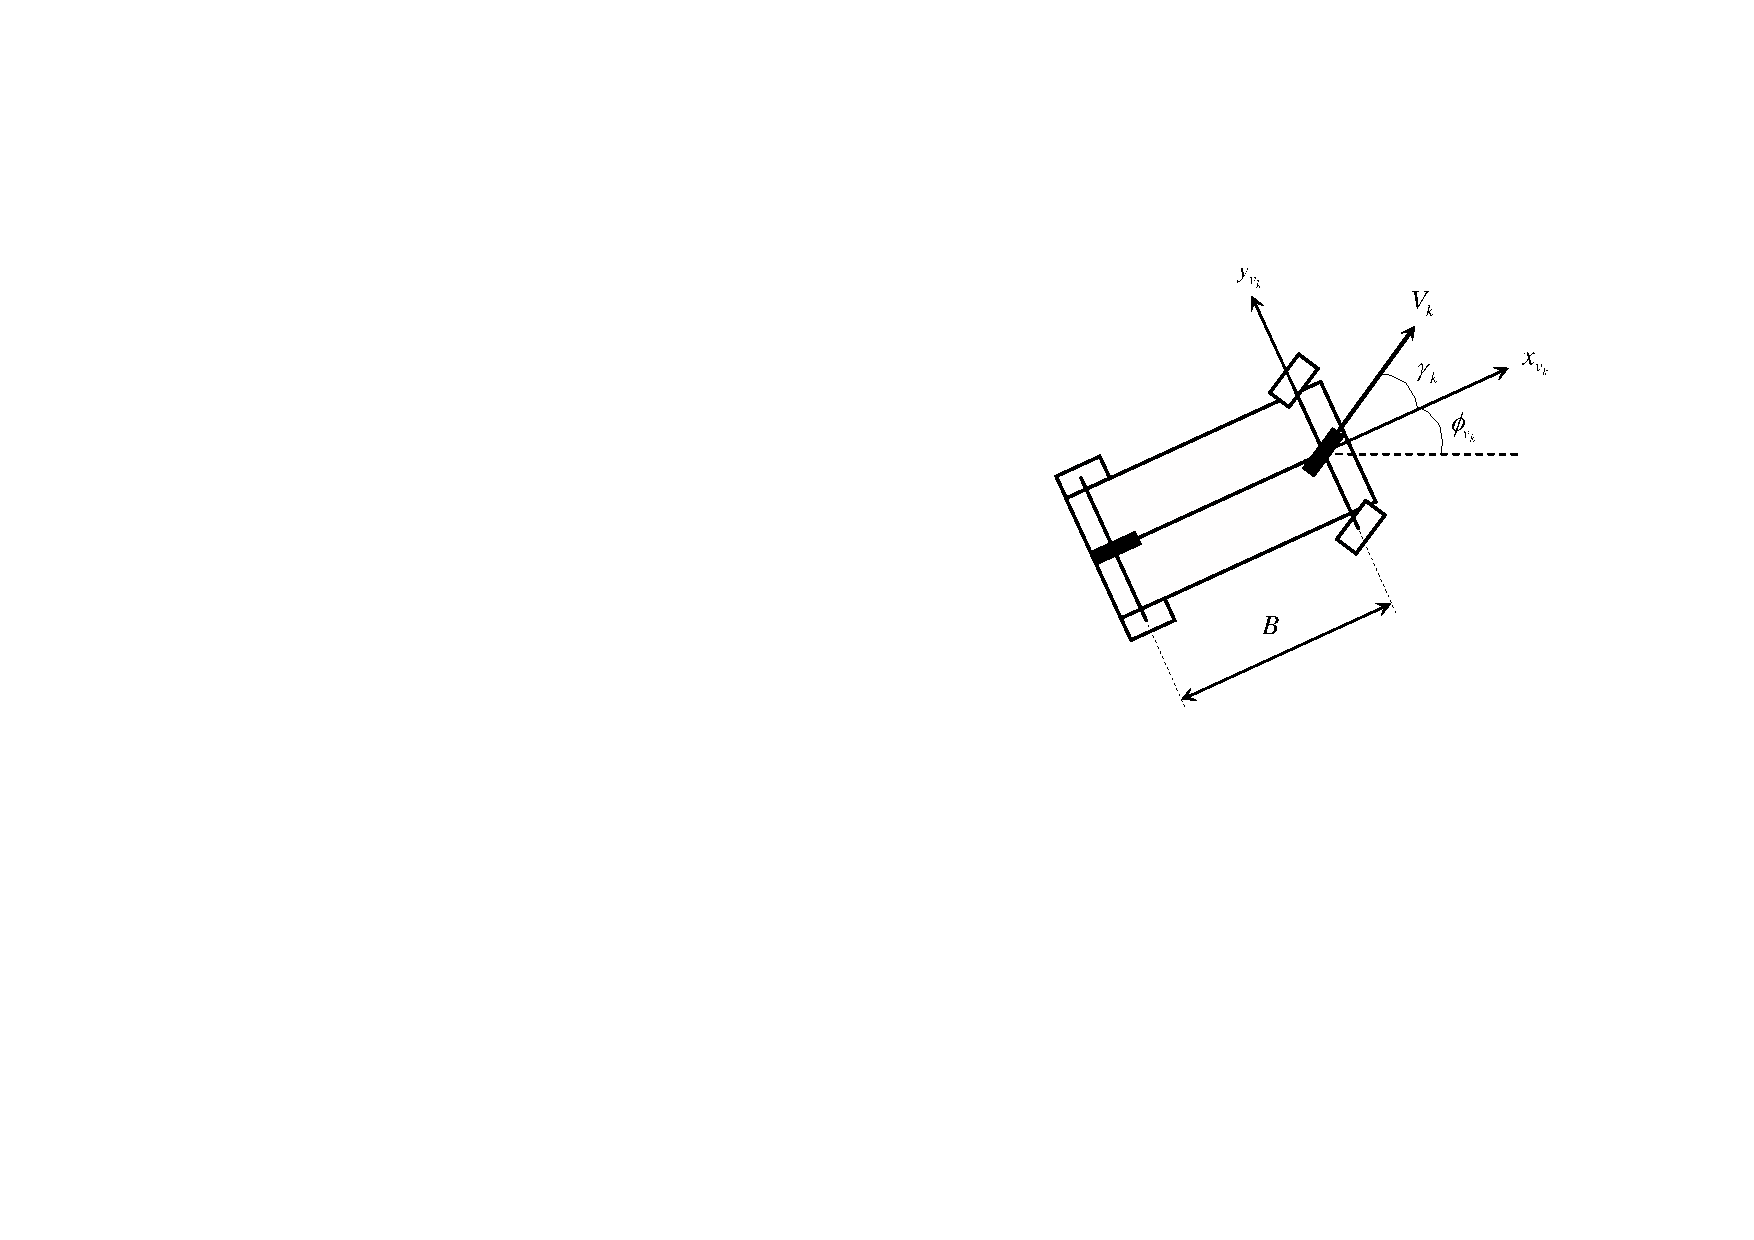
\includegraphics[]{vehmodel}
\caption{Vehicle Motion Model}
\label{f:motion}
\end{center}
\end{figure}


Besides updating the position of the robot in the state vector. We
also want to update the uncertainty of the estimated position of the
robot and the estimated positions of the landmarks. These
uncertainties are stored in a covariance matrix. In matlab code, the
covariance matrix \verb|PX| is updated as follows:

\begin{verbatim}
PX(1:3,1:3)= Gv*PX(1:3,1:3)*Gv' + Gu*Q*Gu';
if size(PX,1)>3
    PX(1:3,4:end)= Gv*PX(1:3,4:end);
    PX(4:end,1:3)= PX(1:3,4:end)';
end 
\end{verbatim}
In the first line, the uncertainty of the robot's xy-position and
orientation is updated. In the next four lines, the uncertainty of the
relation between the robot and all the landmarks in the map are
updated.

To calculate these updates, we need the Jacobians $G_u$ and $G_v$ for
our robot model. The Jacobians are as follows:

\newcommand{\vtc}{V_k \Delta T \cos(\psi_{v_{k-1}} +\gamma_k)}
\newcommand{\vts}{V_k \Delta T \sin(\psi_{v_{k-1}} +\gamma_k)}

\begin{equation}
\mathbf{G}_v=
\left[
\begin{array}{ccc}
1& 0& -\vts \\
0 &1& \vtc\\
0 &0& 1\\
\end{array}
\right]
\end{equation}

\begin{equation}
\mathbf{G}_u=
\left[
\begin{array}{cc}
\Delta T \cos(\psi_{v_{k-1}} +\gamma_k)&  -\vts \\
\Delta T \sin(\psi_{v_{k-1}} +\gamma_k) & \vtc\\
\Delta T \sin(\gamma_k)\over B & V_k\Delta T \cos(\gamma_k)\over B\\
\end{array}
\right]
\end{equation}
where $V_k$ is the velocity control input and $\gamma_k$ is the steering angle input and $B$ is the wheel base of the vehicle and $\psi_{v_{k-1}} $ is orientation from the current head of the SLAM state vector. 


You will need to look through the code. Open \textbf{predict.m} and find how these variables match up with update equations and fill in the empty code. Note \textbf{function angle = pi\_to\_pi(angle)}
should be used when adding headings and steering angles to perform correct modulus wrap around.





\subsection{Observation: Sensor model}
The observation stage consists of a series of observations that arrive
from sensors. In this case, the vehicle is equipped with a laser range
finder. Observations of beacons in the environment can be used to
provide a position estimate when the position of the beacons is
known. This model is depicted in Figure~\ref{f:obmodel}.

To compute the vehicles position from a beacon observation, we need to
calculate the distance and angle towards the beacon:

\begin{figure}[h]
\begin{center}
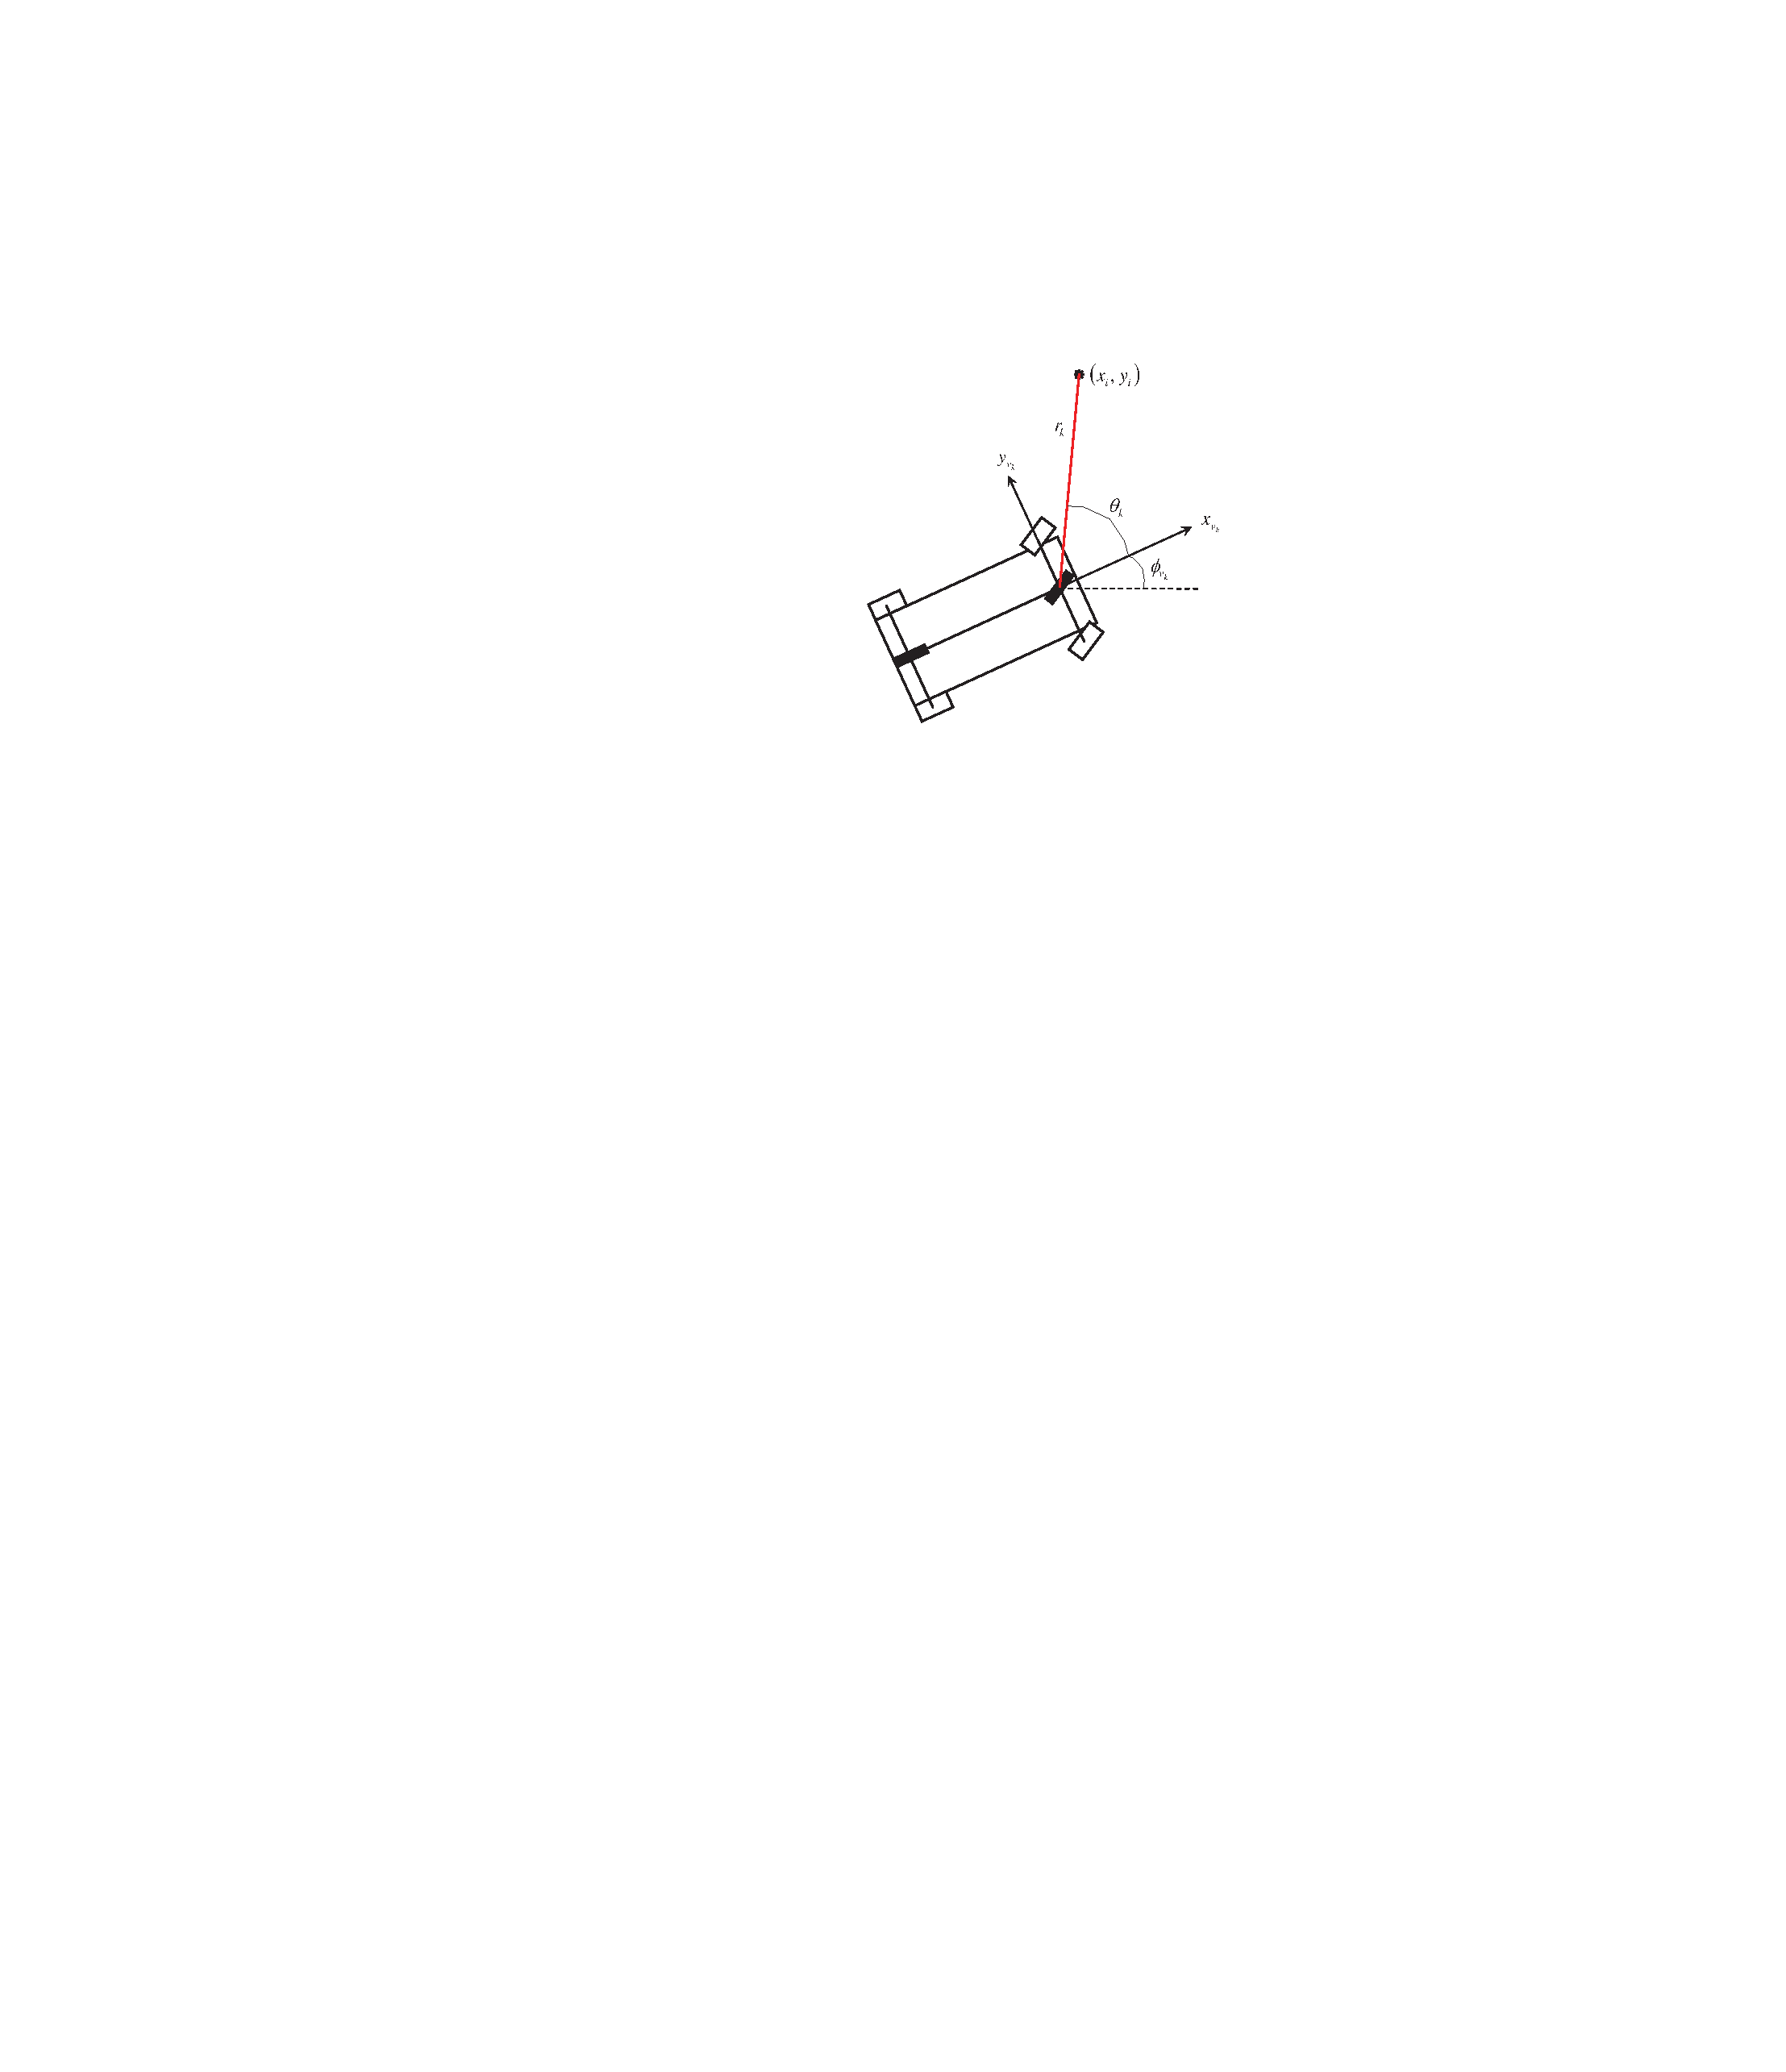
\includegraphics[]{sensormodel}
\caption{Observation Model}
\label{f:obmodel}
\end{center}
\end{figure}

\begin{equation}
\mathbf{z}_{i_k} = \mathbf{h}_i(\mathbf{x}_{k}) = \left[
\begin{array}{c}
\sqrt{(x_i - x_{v_k})^2 + (y_i - y_{v_k})^2}  \\
\mathbf{arctan}\frac{y_i-y_{v_k}}{x_i-x_{v_k}} - \phi_{v_k}\\
\end{array}
\right]
\end{equation}
where $x_i$ and $y_i$ are the x- and y-position of the beacon.

\def \dx {x_i - x_{v_k}}
\def \dy { y_i - y_{v_k}}
\def \d {\sqrt{\ds}}
\def \ds {\left(\dx\right)^2 + \left(\dy\right)^2}
%d= sqrt(d2);
%xd= dx/d;
%yd= dy/d;
%xd2= dx/d2;
%yd2= dy/d2;


The Jacobian of the observation model is :
\begin{equation}
  \frac{\partial h_r}{\partial x} = \left( \begin{array}{ccc}
   -\frac{\dx}{\d} & -\frac{\dy}{\d} & 0  \\
    \frac{\dy}{\ds} & -\frac{\dx}{\ds} & -1
     \end{array} \right) 
      \end{equation}

\begin{equation}
  \frac{\partial h_l}{\partial x} = \left( \begin{array}{cc}
   \frac{\dx}{\d} & \frac{\dy}{\d}  \\
    -\frac{\dy}{\ds} & \frac{\dx}{\ds}
  \end{array} \right) 
\end{equation}
where $\frac{\partial h_r}{\partial x} $is the jacobian for the robot and 
$\frac{\partial h_r}{\partial x}$ is the jacobian for the landmark.

       
You will need to look through the code. Open
\textbf{observe\_model.m} and find how these variables match up
with observation equations and fill in the empty code. Hint:
$H$ is a matrix of size 2 x (length of state vector) and $\frac{\partial
  h_r}{\partial x} $ is the top of the H matrix and $\frac{\partial
  h_l}{\partial x}$ is stored in \verb|H(:,fpos:fpos+1)| positions
calculated in the code. And the index \textbf{fpos} in the
state vector \textbf{x} is the position of the landmark
$(x_i,y_i)$

\section{Running}
Once the functions have been filled in you can run the EKF slam simulator as follows:
\begin{verbatim}
load example_webmap;
ekfslam_sim(lm,wp);

\end{verbatim}

After you have successfully run the example run \textbf{frontend.m} and create a map where the landmarks are spaced quite far apart along the trajectory and watch how the true path and estimated path diverge. Note the effect of landmark placement on the successful localization of the vehicle.

\end{document}
